% Options for packages loaded elsewhere
\PassOptionsToPackage{unicode}{hyperref}
\PassOptionsToPackage{hyphens}{url}
%
\documentclass[
]{article}
\usepackage{amsmath,amssymb}
\usepackage{lmodern}
\usepackage{iftex}
\ifPDFTeX
  \usepackage[T1]{fontenc}
  \usepackage[utf8]{inputenc}
  \usepackage{textcomp} % provide euro and other symbols
\else % if luatex or xetex
  \usepackage{unicode-math}
  \defaultfontfeatures{Scale=MatchLowercase}
  \defaultfontfeatures[\rmfamily]{Ligatures=TeX,Scale=1}
\fi
% Use upquote if available, for straight quotes in verbatim environments
\IfFileExists{upquote.sty}{\usepackage{upquote}}{}
\IfFileExists{microtype.sty}{% use microtype if available
  \usepackage[]{microtype}
  \UseMicrotypeSet[protrusion]{basicmath} % disable protrusion for tt fonts
}{}
\makeatletter
\@ifundefined{KOMAClassName}{% if non-KOMA class
  \IfFileExists{parskip.sty}{%
    \usepackage{parskip}
  }{% else
    \setlength{\parindent}{0pt}
    \setlength{\parskip}{6pt plus 2pt minus 1pt}}
}{% if KOMA class
  \KOMAoptions{parskip=half}}
\makeatother
\usepackage{xcolor}
\usepackage[margin=1in]{geometry}
\usepackage{color}
\usepackage{fancyvrb}
\newcommand{\VerbBar}{|}
\newcommand{\VERB}{\Verb[commandchars=\\\{\}]}
\DefineVerbatimEnvironment{Highlighting}{Verbatim}{commandchars=\\\{\}}
% Add ',fontsize=\small' for more characters per line
\usepackage{framed}
\definecolor{shadecolor}{RGB}{248,248,248}
\newenvironment{Shaded}{\begin{snugshade}}{\end{snugshade}}
\newcommand{\AlertTok}[1]{\textcolor[rgb]{0.94,0.16,0.16}{#1}}
\newcommand{\AnnotationTok}[1]{\textcolor[rgb]{0.56,0.35,0.01}{\textbf{\textit{#1}}}}
\newcommand{\AttributeTok}[1]{\textcolor[rgb]{0.77,0.63,0.00}{#1}}
\newcommand{\BaseNTok}[1]{\textcolor[rgb]{0.00,0.00,0.81}{#1}}
\newcommand{\BuiltInTok}[1]{#1}
\newcommand{\CharTok}[1]{\textcolor[rgb]{0.31,0.60,0.02}{#1}}
\newcommand{\CommentTok}[1]{\textcolor[rgb]{0.56,0.35,0.01}{\textit{#1}}}
\newcommand{\CommentVarTok}[1]{\textcolor[rgb]{0.56,0.35,0.01}{\textbf{\textit{#1}}}}
\newcommand{\ConstantTok}[1]{\textcolor[rgb]{0.00,0.00,0.00}{#1}}
\newcommand{\ControlFlowTok}[1]{\textcolor[rgb]{0.13,0.29,0.53}{\textbf{#1}}}
\newcommand{\DataTypeTok}[1]{\textcolor[rgb]{0.13,0.29,0.53}{#1}}
\newcommand{\DecValTok}[1]{\textcolor[rgb]{0.00,0.00,0.81}{#1}}
\newcommand{\DocumentationTok}[1]{\textcolor[rgb]{0.56,0.35,0.01}{\textbf{\textit{#1}}}}
\newcommand{\ErrorTok}[1]{\textcolor[rgb]{0.64,0.00,0.00}{\textbf{#1}}}
\newcommand{\ExtensionTok}[1]{#1}
\newcommand{\FloatTok}[1]{\textcolor[rgb]{0.00,0.00,0.81}{#1}}
\newcommand{\FunctionTok}[1]{\textcolor[rgb]{0.00,0.00,0.00}{#1}}
\newcommand{\ImportTok}[1]{#1}
\newcommand{\InformationTok}[1]{\textcolor[rgb]{0.56,0.35,0.01}{\textbf{\textit{#1}}}}
\newcommand{\KeywordTok}[1]{\textcolor[rgb]{0.13,0.29,0.53}{\textbf{#1}}}
\newcommand{\NormalTok}[1]{#1}
\newcommand{\OperatorTok}[1]{\textcolor[rgb]{0.81,0.36,0.00}{\textbf{#1}}}
\newcommand{\OtherTok}[1]{\textcolor[rgb]{0.56,0.35,0.01}{#1}}
\newcommand{\PreprocessorTok}[1]{\textcolor[rgb]{0.56,0.35,0.01}{\textit{#1}}}
\newcommand{\RegionMarkerTok}[1]{#1}
\newcommand{\SpecialCharTok}[1]{\textcolor[rgb]{0.00,0.00,0.00}{#1}}
\newcommand{\SpecialStringTok}[1]{\textcolor[rgb]{0.31,0.60,0.02}{#1}}
\newcommand{\StringTok}[1]{\textcolor[rgb]{0.31,0.60,0.02}{#1}}
\newcommand{\VariableTok}[1]{\textcolor[rgb]{0.00,0.00,0.00}{#1}}
\newcommand{\VerbatimStringTok}[1]{\textcolor[rgb]{0.31,0.60,0.02}{#1}}
\newcommand{\WarningTok}[1]{\textcolor[rgb]{0.56,0.35,0.01}{\textbf{\textit{#1}}}}
\usepackage{graphicx}
\makeatletter
\def\maxwidth{\ifdim\Gin@nat@width>\linewidth\linewidth\else\Gin@nat@width\fi}
\def\maxheight{\ifdim\Gin@nat@height>\textheight\textheight\else\Gin@nat@height\fi}
\makeatother
% Scale images if necessary, so that they will not overflow the page
% margins by default, and it is still possible to overwrite the defaults
% using explicit options in \includegraphics[width, height, ...]{}
\setkeys{Gin}{width=\maxwidth,height=\maxheight,keepaspectratio}
% Set default figure placement to htbp
\makeatletter
\def\fps@figure{htbp}
\makeatother
\setlength{\emergencystretch}{3em} % prevent overfull lines
\providecommand{\tightlist}{%
  \setlength{\itemsep}{0pt}\setlength{\parskip}{0pt}}
\setcounter{secnumdepth}{-\maxdimen} % remove section numbering
\ifLuaTeX
  \usepackage{selnolig}  % disable illegal ligatures
\fi
\IfFileExists{bookmark.sty}{\usepackage{bookmark}}{\usepackage{hyperref}}
\IfFileExists{xurl.sty}{\usepackage{xurl}}{} % add URL line breaks if available
\urlstyle{same} % disable monospaced font for URLs
\hypersetup{
  pdftitle={Assignment 1: Cinema},
  pdfauthor={Ian Lacy},
  hidelinks,
  pdfcreator={LaTeX via pandoc}}

\title{Assignment 1: Cinema}
\author{Ian Lacy}
\date{2023-09-27}

\begin{document}
\maketitle

\begin{Shaded}
\begin{Highlighting}[]
\FunctionTok{suppressMessages}\NormalTok{(}\FunctionTok{library}\NormalTok{(readr))}
\FunctionTok{suppressMessages}\NormalTok{(}\FunctionTok{library}\NormalTok{(ggplot2))}
\FunctionTok{suppressMessages}\NormalTok{(}\FunctionTok{library}\NormalTok{(caret))}
\end{Highlighting}
\end{Shaded}

\begin{Shaded}
\begin{Highlighting}[]
\FunctionTok{suppressMessages}\NormalTok{(}\FunctionTok{library}\NormalTok{(tidyr))}
\FunctionTok{suppressMessages}\NormalTok{(}\FunctionTok{library}\NormalTok{(dplyr))}
\FunctionTok{suppressMessages}\NormalTok{(}\FunctionTok{library}\NormalTok{(reshape2))}
\end{Highlighting}
\end{Shaded}

\begin{Shaded}
\begin{Highlighting}[]
\NormalTok{MovieStuff }\OtherTok{\textless{}{-}} \FunctionTok{read\_csv}\NormalTok{(}\StringTok{"C:/Users/ianla.000/Downloads/cinema.csv"}\NormalTok{)}
\end{Highlighting}
\end{Shaded}

\begin{verbatim}
## New names:
## Rows: 61 Columns: 256
## -- Column specification
## -------------------------------------------------------- Delimiter: "," chr
## (1): co-productions dbl (8): year, total, Portugal, Spain, France, UK, USA,
## other_countries lgl (247): ...10, ...11, ...12, ...13, ...14, ...15, ...16,
## ...17, ...18, .....
## i Use `spec()` to retrieve the full column specification for this data. i
## Specify the column types or set `show_col_types = FALSE` to quiet this message.
## * `` -> `...10`
## * `` -> `...11`
## * `` -> `...12`
## * `` -> `...13`
## * `` -> `...14`
## * `` -> `...15`
## * `` -> `...16`
## * `` -> `...17`
## * `` -> `...18`
## * `` -> `...19`
## * `` -> `...20`
## * `` -> `...21`
## * `` -> `...22`
## * `` -> `...23`
## * `` -> `...24`
## * `` -> `...25`
## * `` -> `...26`
## * `` -> `...27`
## * `` -> `...28`
## * `` -> `...29`
## * `` -> `...30`
## * `` -> `...31`
## * `` -> `...32`
## * `` -> `...33`
## * `` -> `...34`
## * `` -> `...35`
## * `` -> `...36`
## * `` -> `...37`
## * `` -> `...38`
## * `` -> `...39`
## * `` -> `...40`
## * `` -> `...41`
## * `` -> `...42`
## * `` -> `...43`
## * `` -> `...44`
## * `` -> `...45`
## * `` -> `...46`
## * `` -> `...47`
## * `` -> `...48`
## * `` -> `...49`
## * `` -> `...50`
## * `` -> `...51`
## * `` -> `...52`
## * `` -> `...53`
## * `` -> `...54`
## * `` -> `...55`
## * `` -> `...56`
## * `` -> `...57`
## * `` -> `...58`
## * `` -> `...59`
## * `` -> `...60`
## * `` -> `...61`
## * `` -> `...62`
## * `` -> `...63`
## * `` -> `...64`
## * `` -> `...65`
## * `` -> `...66`
## * `` -> `...67`
## * `` -> `...68`
## * `` -> `...69`
## * `` -> `...70`
## * `` -> `...71`
## * `` -> `...72`
## * `` -> `...73`
## * `` -> `...74`
## * `` -> `...75`
## * `` -> `...76`
## * `` -> `...77`
## * `` -> `...78`
## * `` -> `...79`
## * `` -> `...80`
## * `` -> `...81`
## * `` -> `...82`
## * `` -> `...83`
## * `` -> `...84`
## * `` -> `...85`
## * `` -> `...86`
## * `` -> `...87`
## * `` -> `...88`
## * `` -> `...89`
## * `` -> `...90`
## * `` -> `...91`
## * `` -> `...92`
## * `` -> `...93`
## * `` -> `...94`
## * `` -> `...95`
## * `` -> `...96`
## * `` -> `...97`
## * `` -> `...98`
## * `` -> `...99`
## * `` -> `...100`
## * `` -> `...101`
## * `` -> `...102`
## * `` -> `...103`
## * `` -> `...104`
## * `` -> `...105`
## * `` -> `...106`
## * `` -> `...107`
## * `` -> `...108`
## * `` -> `...109`
## * `` -> `...110`
## * `` -> `...111`
## * `` -> `...112`
## * `` -> `...113`
## * `` -> `...114`
## * `` -> `...115`
## * `` -> `...116`
## * `` -> `...117`
## * `` -> `...118`
## * `` -> `...119`
## * `` -> `...120`
## * `` -> `...121`
## * `` -> `...122`
## * `` -> `...123`
## * `` -> `...124`
## * `` -> `...125`
## * `` -> `...126`
## * `` -> `...127`
## * `` -> `...128`
## * `` -> `...129`
## * `` -> `...130`
## * `` -> `...131`
## * `` -> `...132`
## * `` -> `...133`
## * `` -> `...134`
## * `` -> `...135`
## * `` -> `...136`
## * `` -> `...137`
## * `` -> `...138`
## * `` -> `...139`
## * `` -> `...140`
## * `` -> `...141`
## * `` -> `...142`
## * `` -> `...143`
## * `` -> `...144`
## * `` -> `...145`
## * `` -> `...146`
## * `` -> `...147`
## * `` -> `...148`
## * `` -> `...149`
## * `` -> `...150`
## * `` -> `...151`
## * `` -> `...152`
## * `` -> `...153`
## * `` -> `...154`
## * `` -> `...155`
## * `` -> `...156`
## * `` -> `...157`
## * `` -> `...158`
## * `` -> `...159`
## * `` -> `...160`
## * `` -> `...161`
## * `` -> `...162`
## * `` -> `...163`
## * `` -> `...164`
## * `` -> `...165`
## * `` -> `...166`
## * `` -> `...167`
## * `` -> `...168`
## * `` -> `...169`
## * `` -> `...170`
## * `` -> `...171`
## * `` -> `...172`
## * `` -> `...173`
## * `` -> `...174`
## * `` -> `...175`
## * `` -> `...176`
## * `` -> `...177`
## * `` -> `...178`
## * `` -> `...179`
## * `` -> `...180`
## * `` -> `...181`
## * `` -> `...182`
## * `` -> `...183`
## * `` -> `...184`
## * `` -> `...185`
## * `` -> `...186`
## * `` -> `...187`
## * `` -> `...188`
## * `` -> `...189`
## * `` -> `...190`
## * `` -> `...191`
## * `` -> `...192`
## * `` -> `...193`
## * `` -> `...194`
## * `` -> `...195`
## * `` -> `...196`
## * `` -> `...197`
## * `` -> `...198`
## * `` -> `...199`
## * `` -> `...200`
## * `` -> `...201`
## * `` -> `...202`
## * `` -> `...203`
## * `` -> `...204`
## * `` -> `...205`
## * `` -> `...206`
## * `` -> `...207`
## * `` -> `...208`
## * `` -> `...209`
## * `` -> `...210`
## * `` -> `...211`
## * `` -> `...212`
## * `` -> `...213`
## * `` -> `...214`
## * `` -> `...215`
## * `` -> `...216`
## * `` -> `...217`
## * `` -> `...218`
## * `` -> `...219`
## * `` -> `...220`
## * `` -> `...221`
## * `` -> `...222`
## * `` -> `...223`
## * `` -> `...224`
## * `` -> `...225`
## * `` -> `...226`
## * `` -> `...227`
## * `` -> `...228`
## * `` -> `...229`
## * `` -> `...230`
## * `` -> `...231`
## * `` -> `...232`
## * `` -> `...233`
## * `` -> `...234`
## * `` -> `...235`
## * `` -> `...236`
## * `` -> `...237`
## * `` -> `...238`
## * `` -> `...239`
## * `` -> `...240`
## * `` -> `...241`
## * `` -> `...242`
## * `` -> `...243`
## * `` -> `...244`
## * `` -> `...245`
## * `` -> `...246`
## * `` -> `...247`
## * `` -> `...248`
## * `` -> `...249`
## * `` -> `...250`
## * `` -> `...251`
## * `` -> `...252`
## * `` -> `...253`
## * `` -> `...254`
## * `` -> `...255`
## * `` -> `...256`
\end{verbatim}

\begin{Shaded}
\begin{Highlighting}[]
\NormalTok{MovieStuff2 }\OtherTok{\textless{}{-}}\NormalTok{ MovieStuff[}\DecValTok{1}\SpecialCharTok{:}\DecValTok{40}\NormalTok{,}\DecValTok{1}\SpecialCharTok{:}\DecValTok{9}\NormalTok{]}
\CommentTok{\#MovieStuff2}
\end{Highlighting}
\end{Shaded}

\begin{Shaded}
\begin{Highlighting}[]
\NormalTok{MovieStuff2}\SpecialCharTok{$}\NormalTok{Spain }\OtherTok{=} \FunctionTok{as.numeric}\NormalTok{(}\FunctionTok{as.character}\NormalTok{(MovieStuff2}\SpecialCharTok{$}\NormalTok{Spain))}
\CommentTok{\#MovieStuff2}
\end{Highlighting}
\end{Shaded}

\begin{Shaded}
\begin{Highlighting}[]
\NormalTok{cbbPalette }\OtherTok{\textless{}{-}} \FunctionTok{c}\NormalTok{(}\StringTok{"\#000000"}\NormalTok{, }\StringTok{"\#E69F00"}\NormalTok{, }\StringTok{"\#56B4E9"}\NormalTok{, }\StringTok{"\#009E73"}\NormalTok{, }\StringTok{"\#F0E442"}\NormalTok{, }\StringTok{"\#0072B2"}\NormalTok{, }\StringTok{"\#D55E00"}\NormalTok{, }\StringTok{"\#CC79A7"}\NormalTok{)}
\end{Highlighting}
\end{Shaded}

\begin{Shaded}
\begin{Highlighting}[]
\NormalTok{plot1 }\OtherTok{\textless{}{-}} \FunctionTok{ggplot}\NormalTok{(MovieStuff2, }\FunctionTok{aes}\NormalTok{(}\AttributeTok{x=}\NormalTok{year, }\AttributeTok{y=}\NormalTok{total)) }\SpecialCharTok{+} 
  \FunctionTok{geom\_line}\NormalTok{()}\SpecialCharTok{+}
  \FunctionTok{geom\_point}\NormalTok{() }\SpecialCharTok{+}
\FunctionTok{scale\_x\_continuous}\NormalTok{(}\AttributeTok{n.breaks =}\DecValTok{10}\NormalTok{)}\SpecialCharTok{+}
  \FunctionTok{scale\_y\_continuous}\NormalTok{(}\AttributeTok{n.breaks =} \DecValTok{20}\NormalTok{)}\SpecialCharTok{+}
   \FunctionTok{scale\_colour\_manual}\NormalTok{(}\AttributeTok{values=}\NormalTok{cbbPalette)}\SpecialCharTok{+}
  \FunctionTok{ggtitle}\NormalTok{(}\StringTok{"Total Number of Productions from Selected Countries from 1979 to 2018"}\NormalTok{) }\SpecialCharTok{+}
  \FunctionTok{xlab}\NormalTok{(}\StringTok{"Year"}\NormalTok{) }\SpecialCharTok{+} \FunctionTok{ylab}\NormalTok{(}\StringTok{"Number of Productions"}\NormalTok{)}\SpecialCharTok{+}
  \FunctionTok{theme}\NormalTok{(}\AttributeTok{plot.title =} \FunctionTok{element\_text}\NormalTok{(}\AttributeTok{hjust=}\FloatTok{0.5}\NormalTok{))}
  

\NormalTok{plot1}
\end{Highlighting}
\end{Shaded}

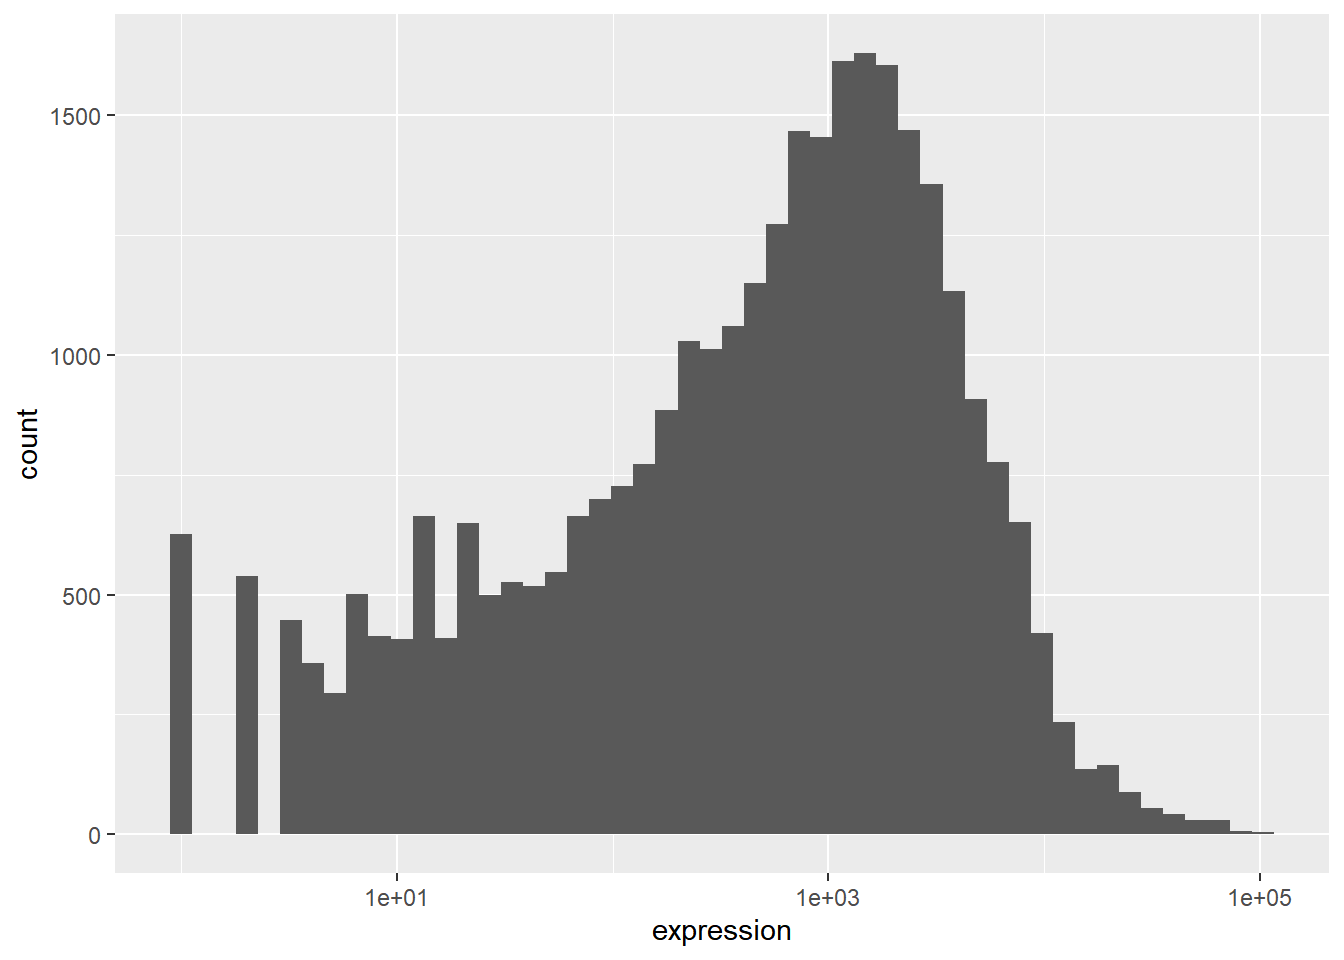
\includegraphics{Assignment-1-DataViz_files/figure-latex/unnamed-chunk-6-1.pdf}
In the above graph all the annual totals for the number of movies
produced per country (Portugal, Spain, UK, USA, France, and a catch all
category called Other Countries). The graph shows that beginning in 1979
the global number of films decreased until 1994 and then nearly
quadrupled from 1995 until 2010. The annual number of total films
produced has remained between 550 and 650 ever since.

\begin{Shaded}
\begin{Highlighting}[]
\NormalTok{plot2 }\OtherTok{\textless{}{-}}\FunctionTok{ggplot}\NormalTok{(MovieStuff2, }\FunctionTok{aes}\NormalTok{(}\AttributeTok{x=}\NormalTok{year, }\AttributeTok{y=}\NormalTok{Portugal)) }\SpecialCharTok{+} 
  \FunctionTok{geom\_line}\NormalTok{()}\SpecialCharTok{+}
  \FunctionTok{geom\_point}\NormalTok{() }\SpecialCharTok{+}
\FunctionTok{scale\_x\_continuous}\NormalTok{(}\AttributeTok{n.breaks =}\DecValTok{10}\NormalTok{)}\SpecialCharTok{+}
  \FunctionTok{scale\_y\_continuous}\NormalTok{(}\AttributeTok{n.breaks =} \DecValTok{10}\NormalTok{)}\SpecialCharTok{+}
  \FunctionTok{scale\_colour\_manual}\NormalTok{(}\AttributeTok{values=}\NormalTok{cbbPalette)}\SpecialCharTok{+}
  \FunctionTok{ggtitle}\NormalTok{(}\StringTok{"Total Number of Productions from Portugal from 1979 to 2018"}\NormalTok{) }\SpecialCharTok{+}
  \FunctionTok{xlab}\NormalTok{(}\StringTok{"Year"}\NormalTok{) }\SpecialCharTok{+} \FunctionTok{ylab}\NormalTok{(}\StringTok{"Number of Productions"}\NormalTok{)}\SpecialCharTok{+}
  \FunctionTok{theme}\NormalTok{(}\AttributeTok{plot.title =} \FunctionTok{element\_text}\NormalTok{(}\AttributeTok{hjust=}\FloatTok{0.5}\NormalTok{))}


\NormalTok{plot2}
\end{Highlighting}
\end{Shaded}

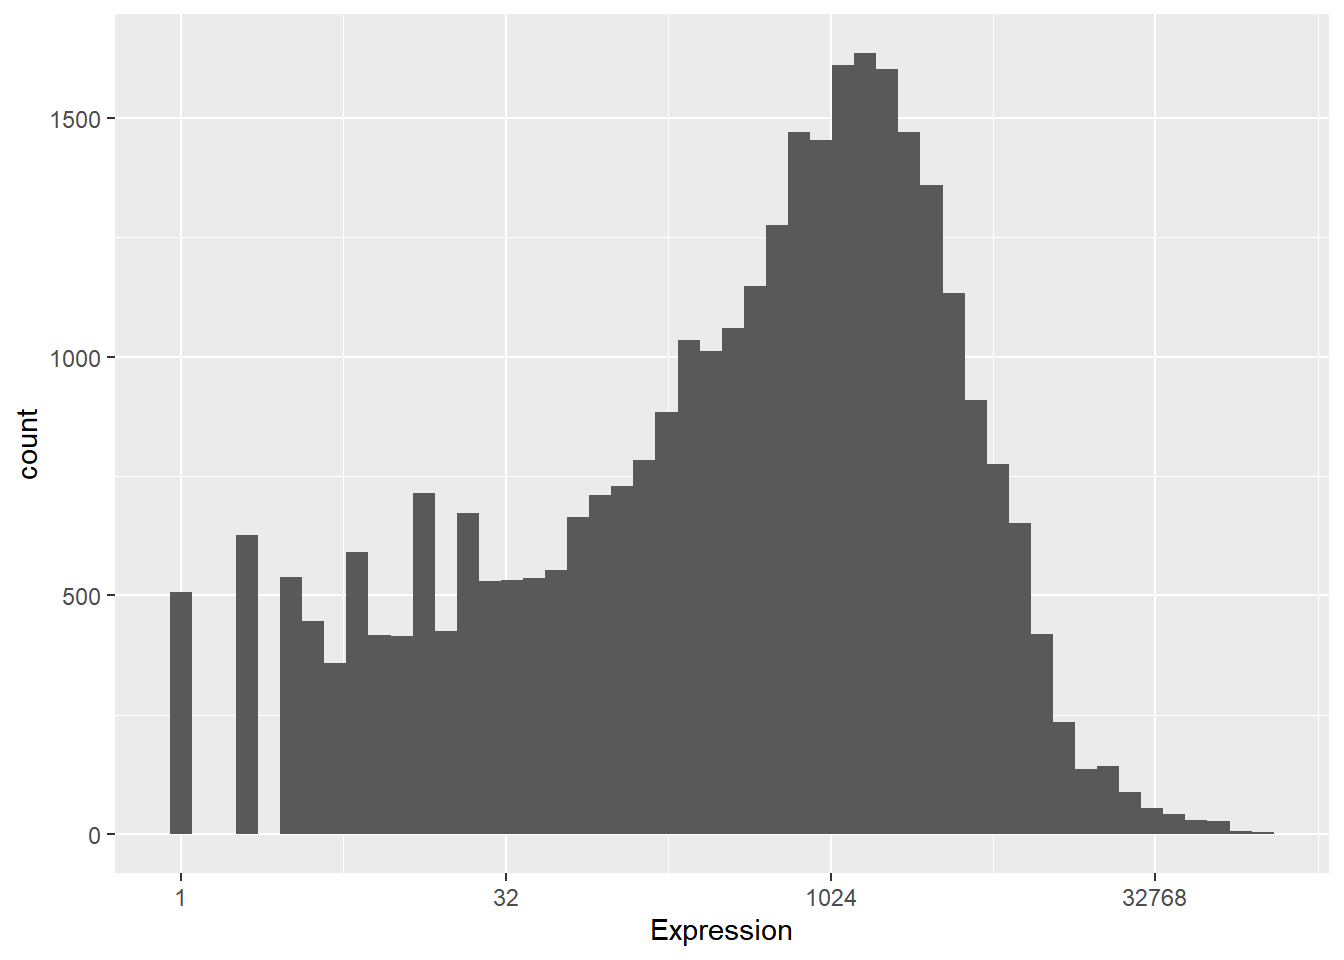
\includegraphics{Assignment-1-DataViz_files/figure-latex/unnamed-chunk-7-1.pdf}

In the above graph all the annual totals for the number of movies
produced in Portugal from 1979 to 2018. The graph shows that the number
of films decreased precipitously from a peak of more than 45 to about 3
per year in 1995. Since 1995, the annual totals have generally trended
up ward apart from yearly changes in the total numbers of movies
produced.

\begin{Shaded}
\begin{Highlighting}[]
\NormalTok{Movies3 }\OtherTok{\textless{}{-}}\NormalTok{ MovieStuff2 }\SpecialCharTok{\%\textgreater{}\%} \FunctionTok{pivot\_longer}\NormalTok{(}\AttributeTok{cols =} \FunctionTok{c}\NormalTok{(}\StringTok{\textquotesingle{}Spain\textquotesingle{}}\NormalTok{, }\StringTok{\textquotesingle{}France\textquotesingle{}}\NormalTok{, }\StringTok{\textquotesingle{}UK\textquotesingle{}}\NormalTok{, }\StringTok{\textquotesingle{}USA\textquotesingle{}}\NormalTok{),}
    \AttributeTok{names\_to =} \StringTok{\textquotesingle{}country\textquotesingle{}}\NormalTok{,}
    \AttributeTok{values\_to =} \StringTok{\textquotesingle{}productions\textquotesingle{}}\NormalTok{)}


\NormalTok{Movies4 }\OtherTok{\textless{}{-}}\NormalTok{ MovieStuff2 }\SpecialCharTok{\%\textgreater{}\%} \FunctionTok{pivot\_longer}\NormalTok{(}\AttributeTok{cols =} \FunctionTok{c}\NormalTok{(}\StringTok{\textquotesingle{}Portugal\textquotesingle{}}\NormalTok{,}\StringTok{\textquotesingle{}Spain\textquotesingle{}}\NormalTok{, }\StringTok{\textquotesingle{}France\textquotesingle{}}\NormalTok{, }\StringTok{\textquotesingle{}UK\textquotesingle{}}\NormalTok{, }\StringTok{\textquotesingle{}USA\textquotesingle{}}\NormalTok{,}\StringTok{\textquotesingle{}other\_countries\textquotesingle{}}\NormalTok{),}
    \AttributeTok{names\_to =} \StringTok{\textquotesingle{}country\textquotesingle{}}\NormalTok{,}
    \AttributeTok{values\_to =} \StringTok{\textquotesingle{}productions\textquotesingle{}}\NormalTok{)}
\end{Highlighting}
\end{Shaded}

\begin{Shaded}
\begin{Highlighting}[]
\NormalTok{Movies3}
\end{Highlighting}
\end{Shaded}

\begin{verbatim}
## # A tibble: 160 x 7
##     year total Portugal other_countries `co-productions` country productions
##    <dbl> <dbl>    <dbl>           <dbl> <chr>            <chr>         <dbl>
##  1  1979  299.     39.8            82.7 x                Spain          6.72
##  2  1979  299.     39.8            82.7 x                France        37.8 
##  3  1979  299.     39.8            82.7 x                UK            30.0 
##  4  1979  299.     39.8            82.7 x                USA          102.  
##  5  1980  300.     41.3            75.6 x                Spain          5.20
##  6  1980  300.     41.3            75.6 x                France        36.6 
##  7  1980  300.     41.3            75.6 x                UK            28.3 
##  8  1980  300.     41.3            75.6 x                USA          113.  
##  9  1981  308.     45.2            73.6 x                Spain          4.88
## 10  1981  308.     45.2            73.6 x                France        34.3 
## # i 150 more rows
\end{verbatim}

\begin{Shaded}
\begin{Highlighting}[]
\NormalTok{Movies4}
\end{Highlighting}
\end{Shaded}

\begin{verbatim}
## # A tibble: 240 x 5
##     year total `co-productions` country         productions
##    <dbl> <dbl> <chr>            <chr>                 <dbl>
##  1  1979  299. x                Portugal              39.8 
##  2  1979  299. x                Spain                  6.72
##  3  1979  299. x                France                37.8 
##  4  1979  299. x                UK                    30.0 
##  5  1979  299. x                USA                  102.  
##  6  1979  299. x                other_countries       82.7 
##  7  1980  300. x                Portugal              41.3 
##  8  1980  300. x                Spain                  5.20
##  9  1980  300. x                France                36.6 
## 10  1980  300. x                UK                    28.3 
## # i 230 more rows
\end{verbatim}

\begin{Shaded}
\begin{Highlighting}[]
\FunctionTok{ggplot}\NormalTok{(Movies3, }\FunctionTok{aes}\NormalTok{(}\AttributeTok{x=}\NormalTok{year, }\AttributeTok{y=}\NormalTok{productions)) }\SpecialCharTok{+} 
  \FunctionTok{geom\_line}\NormalTok{(}\FunctionTok{aes}\NormalTok{(}\AttributeTok{color=}\NormalTok{country))}\SpecialCharTok{+}
  \FunctionTok{geom\_point}\NormalTok{(}\FunctionTok{aes}\NormalTok{(}\AttributeTok{color=}\NormalTok{country))}\SpecialCharTok{+}
  \FunctionTok{scale\_x\_continuous}\NormalTok{(}\AttributeTok{n.breaks =}\DecValTok{10}\NormalTok{)}\SpecialCharTok{+}
  \FunctionTok{scale\_y\_continuous}\NormalTok{(}\AttributeTok{n.breaks =} \DecValTok{15}\NormalTok{)}\SpecialCharTok{+}
  \FunctionTok{ggtitle}\NormalTok{(}\StringTok{"Comparing Number of Productions from France, Spain, UK, and USA (1979 to 2018)"}\NormalTok{) }\SpecialCharTok{+}
  \FunctionTok{xlab}\NormalTok{(}\StringTok{"Year"}\NormalTok{) }\SpecialCharTok{+} 
  \FunctionTok{ylab}\NormalTok{(}\StringTok{"Number of Productions"}\NormalTok{)}\SpecialCharTok{+}
  \FunctionTok{theme}\NormalTok{(}\AttributeTok{plot.title =} \FunctionTok{element\_text}\NormalTok{(}\AttributeTok{hjust=}\FloatTok{0.5}\NormalTok{))}\SpecialCharTok{+}
  \FunctionTok{scale\_colour\_manual}\NormalTok{(}\AttributeTok{values =}\NormalTok{ cbbPalette, }\AttributeTok{name =} \StringTok{"Country"}\NormalTok{)}
\end{Highlighting}
\end{Shaded}

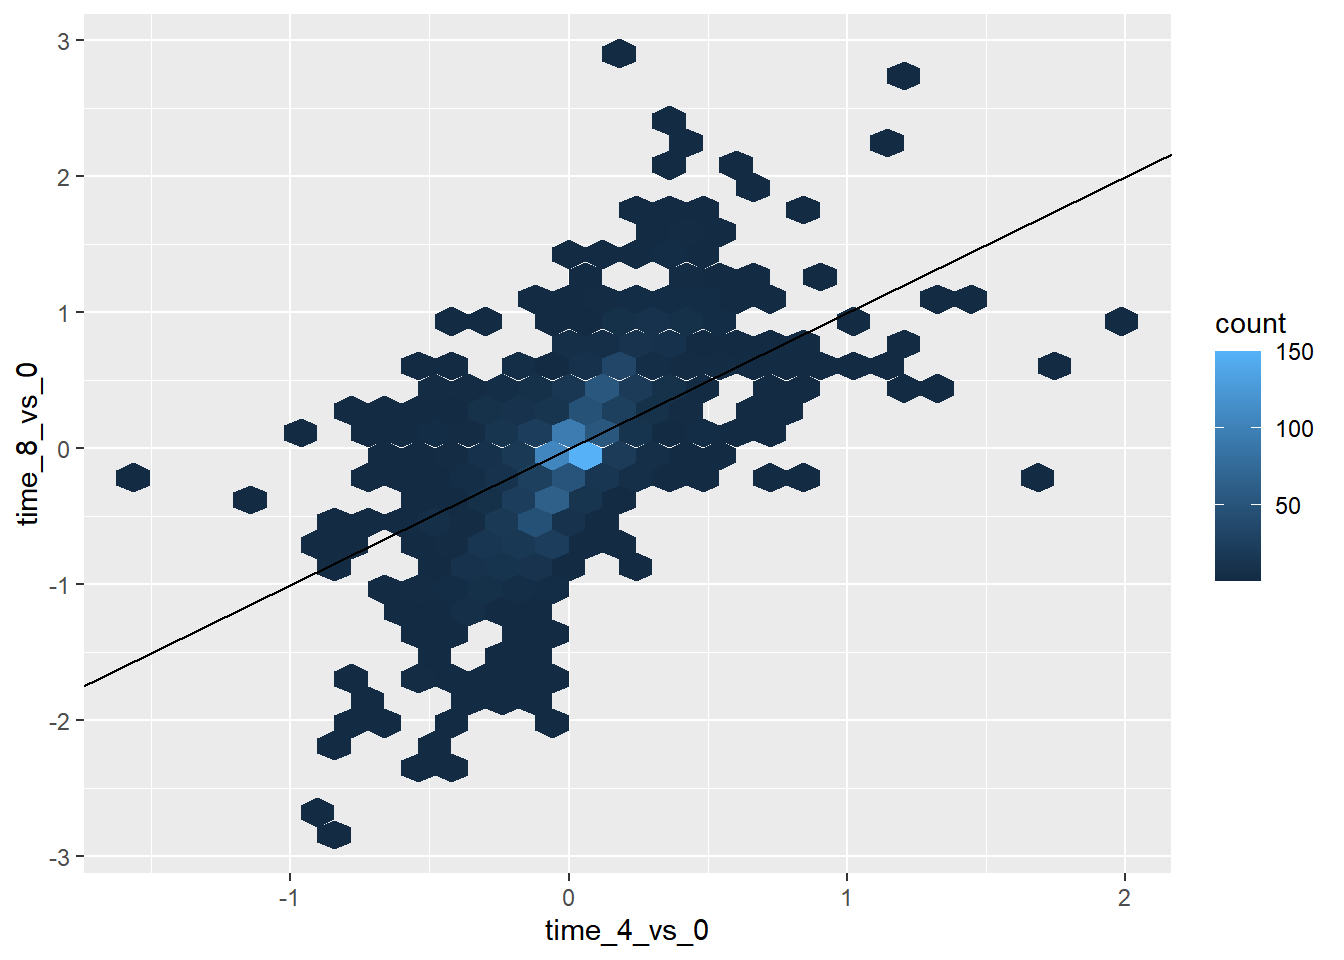
\includegraphics{Assignment-1-DataViz_files/figure-latex/unnamed-chunk-10-1.pdf}
The above graph compares the annual total of movies produced in France,
Spain, UK, and the USA. As we can see France and the UK has produced
under 50 films per year. Spain produced very few films per year until
the 1990s, with a peak of 960 in 1997. Unfortunately, there is no data
about the number of movies produced from 1999 to 2003 and these were
recorded as zero years per year. The USA is the only consistent
producers of movies, with more than 100 movies produced per year from
1979 until 1994. The USA then rapidly increased the number of movies
produced per year from 1994 to 2003. Since 2003, the USA has produced
more than 300 movies per year.

\begin{Shaded}
\begin{Highlighting}[]
\NormalTok{Movies5 }\OtherTok{\textless{}{-}} \FunctionTok{subset}\NormalTok{(Movies4, year }\SpecialCharTok{\%in\%} \FunctionTok{c}\NormalTok{(}\DecValTok{2018}\NormalTok{))}

\NormalTok{Movies5 }\OtherTok{\textless{}{-}} \FunctionTok{select}\NormalTok{(Movies5, }\SpecialCharTok{{-}}\FunctionTok{c}\NormalTok{(}\StringTok{"year"}\NormalTok{,}\StringTok{"total"}\NormalTok{, }\StringTok{"co{-}productions"}\NormalTok{))}
\NormalTok{Movies5}
\end{Highlighting}
\end{Shaded}

\begin{verbatim}
## # A tibble: 6 x 2
##   country         productions
##   <chr>                 <dbl>
## 1 Portugal              14.3 
## 2 Spain                  3.75
## 3 France                20.0 
## 4 UK                    12.9 
## 5 USA                  350.  
## 6 other_countries       18.7
\end{verbatim}

\begin{Shaded}
\begin{Highlighting}[]
\NormalTok{Movies6 }\OtherTok{\textless{}{-}}\NormalTok{ Movies4[Movies4}\SpecialCharTok{$}\NormalTok{country }\SpecialCharTok{\%in\%} \FunctionTok{c}\NormalTok{(}\StringTok{\textquotesingle{}UK\textquotesingle{}}\NormalTok{, }\StringTok{\textquotesingle{}USA\textquotesingle{}}\NormalTok{), ]}
\NormalTok{Movies6 }\OtherTok{\textless{}{-}} \FunctionTok{select}\NormalTok{(Movies6, }\SpecialCharTok{{-}}\FunctionTok{c}\NormalTok{(}\StringTok{"total"}\NormalTok{, }\StringTok{"co{-}productions"}\NormalTok{))}
\NormalTok{Movies6}
\end{Highlighting}
\end{Shaded}

\begin{verbatim}
## # A tibble: 80 x 3
##     year country productions
##    <dbl> <chr>         <dbl>
##  1  1979 UK             30.0
##  2  1979 USA           102. 
##  3  1980 UK             28.3
##  4  1980 USA           113. 
##  5  1981 UK             28.5
##  6  1981 USA           122. 
##  7  1982 UK             26.1
##  8  1982 USA           125. 
##  9  1983 UK             26.2
## 10  1983 USA           124. 
## # i 70 more rows
\end{verbatim}

\begin{Shaded}
\begin{Highlighting}[]
\FunctionTok{ggplot}\NormalTok{(Movies6, }\FunctionTok{aes}\NormalTok{(}\AttributeTok{x=}\NormalTok{year, }\AttributeTok{y=}\NormalTok{productions)) }\SpecialCharTok{+} 
  \FunctionTok{geom\_point}\NormalTok{(}\FunctionTok{aes}\NormalTok{(}\AttributeTok{color=}\NormalTok{country))}\SpecialCharTok{+}
  \FunctionTok{scale\_colour\_manual}\NormalTok{(}\AttributeTok{name =} \StringTok{"Country"}\NormalTok{, }\AttributeTok{values =}\NormalTok{ cbbPalette)}\SpecialCharTok{+}
  \FunctionTok{xlab}\NormalTok{(}\StringTok{"Year"}\NormalTok{) }\SpecialCharTok{+} 
  \FunctionTok{ylab}\NormalTok{(}\StringTok{"Number of Productions"}\NormalTok{)}\SpecialCharTok{+}
  \FunctionTok{ggtitle}\NormalTok{(}\StringTok{"Comparing Number of Productions from UK and USA (1979 to 2018)"}\NormalTok{)}\SpecialCharTok{+}
  \FunctionTok{theme}\NormalTok{(}\AttributeTok{plot.title =} \FunctionTok{element\_text}\NormalTok{(}\AttributeTok{size=} \DecValTok{12}\NormalTok{,}\AttributeTok{hjust=}\FloatTok{0.5}\NormalTok{))}
\end{Highlighting}
\end{Shaded}

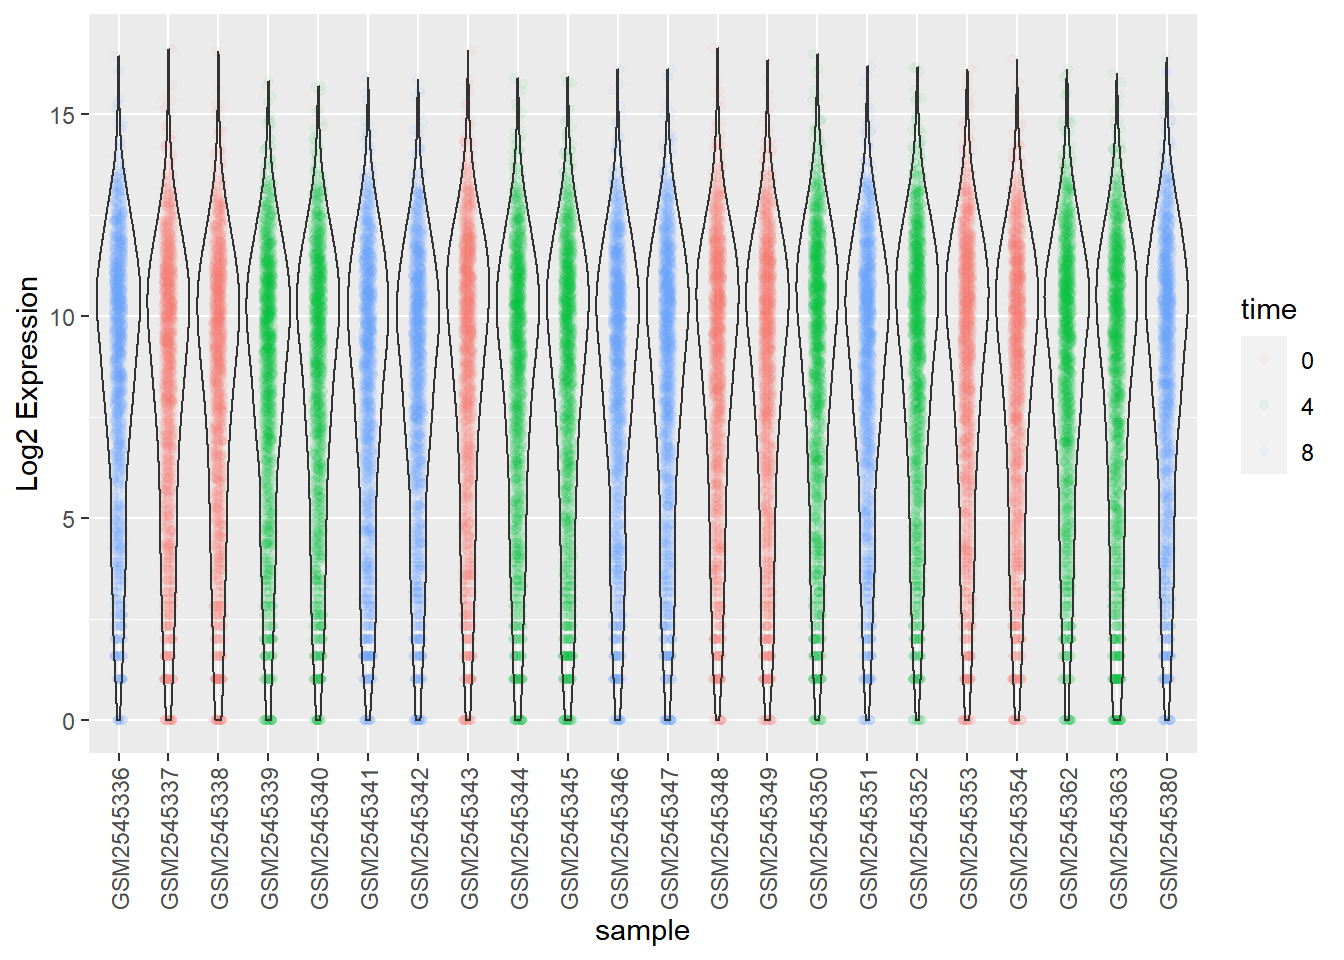
\includegraphics{Assignment-1-DataViz_files/figure-latex/unnamed-chunk-13-1.pdf}

\begin{Shaded}
\begin{Highlighting}[]
\NormalTok{Movies7 }\OtherTok{\textless{}{-}}\NormalTok{ Movies4[Movies4}\SpecialCharTok{$}\NormalTok{country }\SpecialCharTok{\%in\%} \FunctionTok{c}\NormalTok{(}\StringTok{\textquotesingle{}USA\textquotesingle{}}\NormalTok{, }\StringTok{\textquotesingle{}France\textquotesingle{}}\NormalTok{), ]}
\NormalTok{Movies7 }\OtherTok{\textless{}{-}} \FunctionTok{select}\NormalTok{(Movies7, }\SpecialCharTok{{-}}\FunctionTok{c}\NormalTok{(}\StringTok{"total"}\NormalTok{, }\StringTok{"co{-}productions"}\NormalTok{))}
\CommentTok{\#Movies7}
\end{Highlighting}
\end{Shaded}

\begin{Shaded}
\begin{Highlighting}[]
  \FunctionTok{ggplot}\NormalTok{(Movies7, }\FunctionTok{aes}\NormalTok{(}\AttributeTok{x=}\NormalTok{year, }\AttributeTok{y=}\NormalTok{productions)) }\SpecialCharTok{+} 
  \FunctionTok{geom\_point}\NormalTok{(}\FunctionTok{aes}\NormalTok{(}\AttributeTok{color=}\NormalTok{country))}\SpecialCharTok{+}
  \FunctionTok{scale\_colour\_manual}\NormalTok{(}\AttributeTok{name =} \StringTok{"Country"}\NormalTok{, }\AttributeTok{values =}\NormalTok{ cbbPalette)}\SpecialCharTok{+}
  \FunctionTok{xlab}\NormalTok{(}\StringTok{"Year"}\NormalTok{) }\SpecialCharTok{+} 
  \FunctionTok{ylab}\NormalTok{(}\StringTok{"Number of Productions"}\NormalTok{)}\SpecialCharTok{+}
  \FunctionTok{ggtitle}\NormalTok{(}\StringTok{"Comparing Number of Productions from Franc and USA (1979 to 2018)"}\NormalTok{)}\SpecialCharTok{+}
  \FunctionTok{theme}\NormalTok{(}\AttributeTok{plot.title =} \FunctionTok{element\_text}\NormalTok{(}\AttributeTok{hjust=}\FloatTok{0.5}\NormalTok{))}
\end{Highlighting}
\end{Shaded}

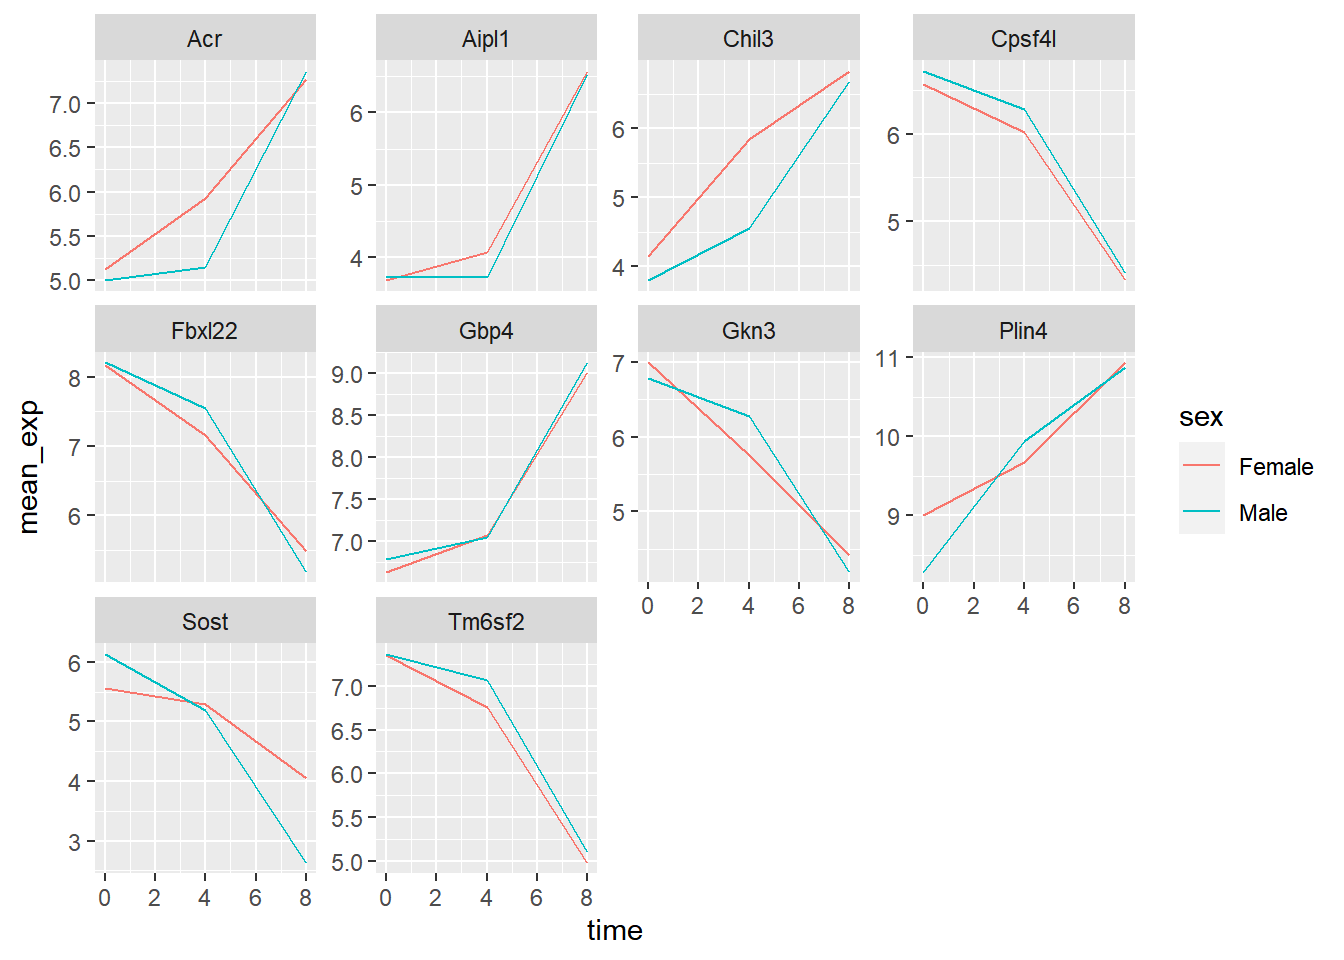
\includegraphics{Assignment-1-DataViz_files/figure-latex/unnamed-chunk-15-1.pdf}

\begin{Shaded}
\begin{Highlighting}[]
\NormalTok{Movies8 }\OtherTok{\textless{}{-}} \FunctionTok{subset}\NormalTok{(Movies4, country }\SpecialCharTok{\%in\%} \FunctionTok{c}\NormalTok{(}\StringTok{"Portugal"}\NormalTok{))}

\NormalTok{Movies8 }\OtherTok{\textless{}{-}} \FunctionTok{select}\NormalTok{(Movies8, }\SpecialCharTok{{-}}\FunctionTok{c}\NormalTok{(}\StringTok{"total"}\NormalTok{, }\StringTok{"co{-}productions"}\NormalTok{))}
\CommentTok{\#Movies8}
\end{Highlighting}
\end{Shaded}

\begin{Shaded}
\begin{Highlighting}[]
\FunctionTok{ggplot}\NormalTok{(Movies8, }\FunctionTok{aes}\NormalTok{(}\AttributeTok{x=}\StringTok{\textquotesingle{}\textquotesingle{}}\NormalTok{, }\AttributeTok{y=}\NormalTok{productions)) }\SpecialCharTok{+}
  \FunctionTok{geom\_boxplot}\NormalTok{(}\FunctionTok{aes}\NormalTok{(}\AttributeTok{fill=}\NormalTok{country))}\SpecialCharTok{+}
  \FunctionTok{scale\_fill\_manual}\NormalTok{(}\AttributeTok{values =} \StringTok{"\#E69F00"}\NormalTok{, }\AttributeTok{name =} \StringTok{"Country"}\NormalTok{)}\SpecialCharTok{+}
  \FunctionTok{xlab}\NormalTok{(}\StringTok{""}\NormalTok{) }\SpecialCharTok{+} 
  \FunctionTok{ylab}\NormalTok{(}\StringTok{"Number of Productions"}\NormalTok{)}\SpecialCharTok{+}
  \FunctionTok{ggtitle}\NormalTok{(}\StringTok{"Distribution of Productions in Portugal (1979 to 2018)"}\NormalTok{)}\SpecialCharTok{+}
  \FunctionTok{theme}\NormalTok{(}\AttributeTok{plot.title =} \FunctionTok{element\_text}\NormalTok{(}\AttributeTok{hjust=}\FloatTok{0.5}\NormalTok{))}
\end{Highlighting}
\end{Shaded}

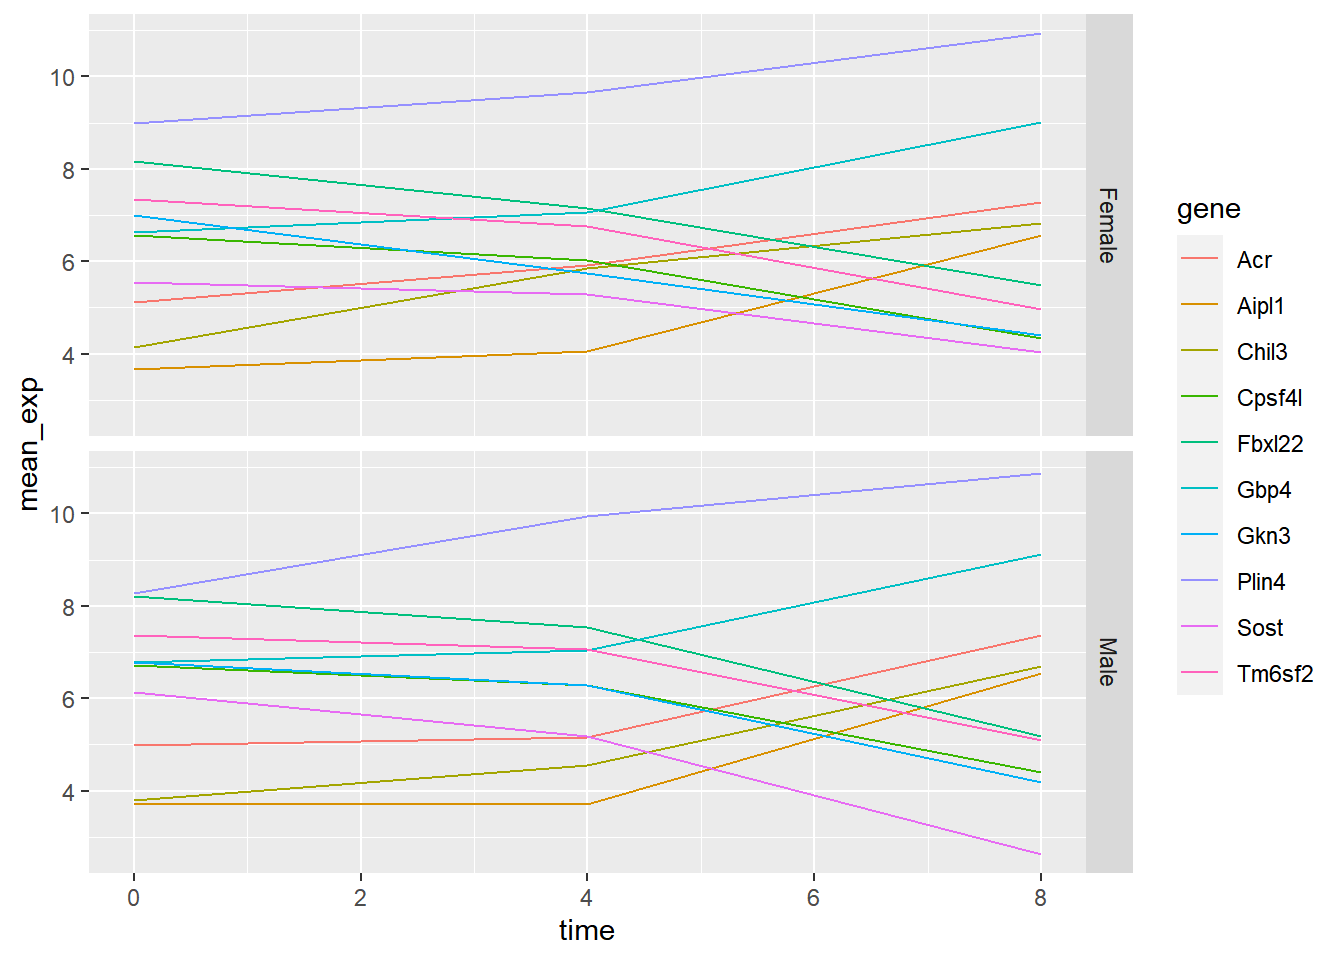
\includegraphics{Assignment-1-DataViz_files/figure-latex/unnamed-chunk-17-1.pdf}

\begin{Shaded}
\begin{Highlighting}[]
\NormalTok{Portugal }\OtherTok{\textless{}{-}}\FunctionTok{sum}\NormalTok{(MovieStuff2}\SpecialCharTok{$}\NormalTok{Portugal)}
\NormalTok{Spain }\OtherTok{\textless{}{-}} \FunctionTok{sum}\NormalTok{(MovieStuff2}\SpecialCharTok{$}\NormalTok{Spain)}
\NormalTok{France }\OtherTok{\textless{}{-}} \FunctionTok{sum}\NormalTok{(MovieStuff2}\SpecialCharTok{$}\NormalTok{France)}
\NormalTok{UK }\OtherTok{\textless{}{-}} \FunctionTok{sum}\NormalTok{(MovieStuff2}\SpecialCharTok{$}\NormalTok{UK)}
\NormalTok{USA }\OtherTok{\textless{}{-}}\FunctionTok{sum}\NormalTok{(MovieStuff2}\SpecialCharTok{$}\NormalTok{USA)}

\NormalTok{GlobalTotal }\OtherTok{\textless{}{-}}\NormalTok{ Portugal}\SpecialCharTok{+}\NormalTok{Spain}\SpecialCharTok{+}\NormalTok{France}\SpecialCharTok{+}\NormalTok{UK}\SpecialCharTok{+}\NormalTok{USA}


\NormalTok{Portugal}
\end{Highlighting}
\end{Shaded}

\begin{verbatim}
## [1] 616.374
\end{verbatim}

\begin{Shaded}
\begin{Highlighting}[]
\NormalTok{Spain}
\end{Highlighting}
\end{Shaded}

\begin{verbatim}
## [1] 4353.35
\end{verbatim}

\begin{Shaded}
\begin{Highlighting}[]
\NormalTok{France}
\end{Highlighting}
\end{Shaded}

\begin{verbatim}
## [1] 569.134
\end{verbatim}

\begin{Shaded}
\begin{Highlighting}[]
\NormalTok{UK}
\end{Highlighting}
\end{Shaded}

\begin{verbatim}
## [1] 565.513
\end{verbatim}

\begin{Shaded}
\begin{Highlighting}[]
\NormalTok{USA}
\end{Highlighting}
\end{Shaded}

\begin{verbatim}
## [1] 10662.62
\end{verbatim}

\begin{Shaded}
\begin{Highlighting}[]
\NormalTok{GlobalTotal}
\end{Highlighting}
\end{Shaded}

\begin{verbatim}
## [1] 16766.99
\end{verbatim}

\begin{Shaded}
\begin{Highlighting}[]
\NormalTok{Produced }\OtherTok{\textless{}{-}} \FunctionTok{c}\NormalTok{(Portugal, Spain, France, UK, USA)}
\NormalTok{Country }\OtherTok{\textless{}{-}} \FunctionTok{c}\NormalTok{(}\StringTok{"Portugal"}\NormalTok{, }\StringTok{"Spain"}\NormalTok{, }\StringTok{"France"}\NormalTok{, }\StringTok{"UK"}\NormalTok{, }\StringTok{"USA"}\NormalTok{)}

\NormalTok{USAVersusTotal }\OtherTok{\textless{}{-}} \FunctionTok{data.frame}\NormalTok{(Produced, Country)}

\NormalTok{USAVersusTotal}
\end{Highlighting}
\end{Shaded}

\begin{verbatim}
##    Produced  Country
## 1   616.374 Portugal
## 2  4353.350    Spain
## 3   569.134   France
## 4   565.513       UK
## 5 10662.620      USA
\end{verbatim}

\begin{Shaded}
\begin{Highlighting}[]
\NormalTok{USAStack }\OtherTok{\textless{}{-}} \FunctionTok{ggplot}\NormalTok{(USAVersusTotal, }\FunctionTok{aes}\NormalTok{(}\AttributeTok{fill=}\NormalTok{Country, }\AttributeTok{y=}\NormalTok{Produced, }\AttributeTok{x=}\StringTok{\textquotesingle{}\textquotesingle{}}\NormalTok{)) }\SpecialCharTok{+} 
  \FunctionTok{geom\_bar}\NormalTok{(}\AttributeTok{position=}\StringTok{"stack"}\NormalTok{, }\AttributeTok{stat=}\StringTok{"identity"}\NormalTok{)}\SpecialCharTok{+}
  \FunctionTok{xlab}\NormalTok{(}\StringTok{""}\NormalTok{) }\SpecialCharTok{+} 
  \FunctionTok{ylab}\NormalTok{(}\StringTok{"Number of Movies Produced"}\NormalTok{)}\SpecialCharTok{+}
  \FunctionTok{ggtitle}\NormalTok{(}\StringTok{"Comparison of Individual Country Production Totals to the Global Total (1979 to 2018)"}\NormalTok{)}\SpecialCharTok{+}
  \FunctionTok{theme}\NormalTok{(}\AttributeTok{plot.title =} \FunctionTok{element\_text}\NormalTok{(}\AttributeTok{hjust=}\FloatTok{0.5}\NormalTok{))}\SpecialCharTok{+}
  \FunctionTok{scale\_fill\_manual}\NormalTok{(}\AttributeTok{values =}\NormalTok{ cbbPalette)}
  



\NormalTok{USAStack }
\end{Highlighting}
\end{Shaded}

\includegraphics{Assignment-1-DataViz_files/figure-latex/unnamed-chunk-19-1.pdf}

\end{document}
